% Updated architecture diagram (2026-11-10), drawn in the style and layout of the proposal's Fig. 1 so the two
% compare directly. Changes vs the proposal: action-conditioned shield rule, shield also uses track walls and the
% car's state, friction-circle tires, stall recovery. Build: tectonic -X compile architecture_v2.tex
\documentclass[border=4pt]{standalone}
\usepackage[T1]{fontenc}
\usepackage{newtxtext,newtxmath}
\usepackage{tikz}
\usetikzlibrary{arrows.meta,positioning,calc}
\begin{document}
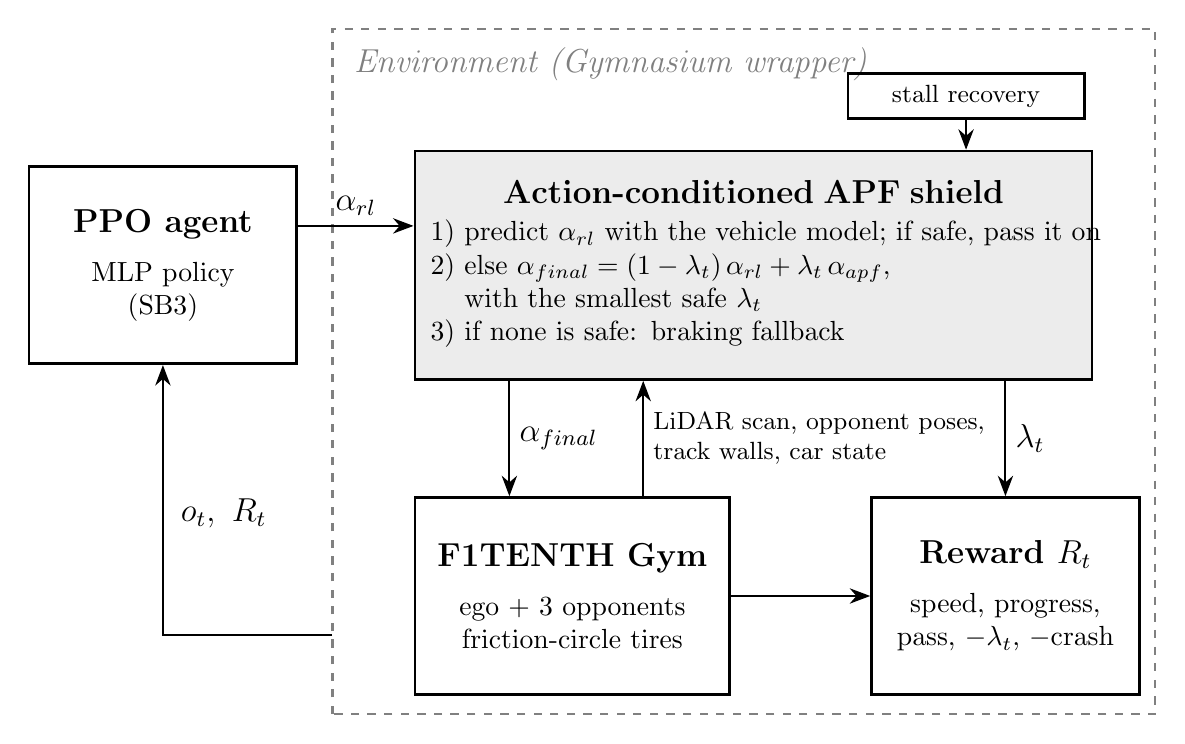
\begin{tikzpicture}[>={Stealth[length=2.6mm]}, line width=0.7pt,
  box/.style={draw, line width=1pt, align=center, inner sep=4pt}]
% environment frame
\draw[dashed, gray, line width=1pt] (3.55,-6.25) rectangle (14.0,2.45);
\node[anchor=north west, gray, font=\itshape\large] at (3.7,2.35) {Environment (Gymnasium wrapper)};
% PPO agent
\node[box, minimum width=3.4cm, minimum height=2.5cm] (ppo) at (1.4,-0.55)
  {{\large\bfseries PPO agent}\\[2mm] MLP policy\\(SB3)};
% shield
\node[box, fill=gray!15, minimum width=8.6cm, minimum height=2.9cm, text width=8.2cm] (sh) at (8.9,-0.55)
  {{\large\bfseries Action-conditioned APF shield}\\[1.5mm]
   \begin{tabular}{@{}r@{\ }l@{}}
   1) & predict $\alpha_{rl}$ with the vehicle model; if safe, pass it on\\
   2) & else $\alpha_{final} = (1-\lambda_t)\,\alpha_{rl} + \lambda_t\,\alpha_{apf}$,\\
      & with the smallest safe $\lambda_t$\\
   3) & if none is safe: braking fallback
   \end{tabular}};
% stall recovery
\node[box, font=\small, minimum width=3.0cm] (rec) at (11.6,1.6) {stall recovery};
% simulator and reward
\node[box, minimum width=4.0cm, minimum height=2.5cm] (sim) at (6.6,-4.75)
  {{\large\bfseries F1TENTH Gym}\\[2mm] ego + 3 opponents\\friction-circle tires};
\node[box, minimum width=3.4cm, minimum height=2.5cm] (rew) at (12.1,-4.75)
  {{\large\bfseries Reward $R_t$}\\[2mm] speed, progress,\\pass, $-\lambda_t$, $-$crash};
% arrows
\draw[->] (ppo.east |- 0,-0.05) -- node[above, font=\large]{$\alpha_{rl}$} (sh.west |- 0,-0.05);
\draw[->] (rec.south) -- (rec.south |- sh.north);
\draw[->] ([xshift=-8mm]sim.north |- sh.south) -- node[right, font=\large]{$\alpha_{final}$} ([xshift=-8mm]sim.north);
\draw[->] ([xshift=9mm]sim.north) -- node[right, align=left, font=\small]{LiDAR scan, opponent poses,\\track walls, car state} ([xshift=9mm]sim.north |- sh.south);
\draw[->] (rew.north |- sh.south) -- node[right, font=\large]{$\lambda_t$} (rew.north);
\draw[->] (sim.east) -- (rew.west);
\draw[->] (3.55,-5.25) -- (1.4,-5.25) -- node[pos=0.45, right=1mm, font=\large]{$o_t,\ R_t$} (ppo.south);
\end{tikzpicture}
\end{document}
